% Drawing 67/05-1 -- folder 67, batch 05, archive page 95 (PDF page 96).
% Transcription: feuillet de dessins, sans un mot ni une formule : neuf sphères tracées à main levée au feutre (noir, brun, vert, orange, bleu), chacune découpée par un réseau d'arcs de grands cercles en régions dont certaines sont hachurées ou coloriées ; la plus grande, en orange, en haut à droite, est coupée par quatre cordes en secteurs, l'un hachuré
% Kind: page of spheres cut by great circles (coloured felt pens). Method 2 (schematic redraw from the facsimile). Status: partial.
% Notes: Drawn on a computer printout; the printout text is left out. Nine spheres at their places on the sheet, each outline an ellipse and every chord ending exactly on its outline (endpoints projected onto it), crossings computed: 1 (left) shaded all over, with its network of wavy arcs; 2 (top centre) two chords crossing, the cap above their crossing hatched, a dashed arc behind; a small closed contour beside it; 3 (centre) two chords crossing, the top cap hatched, a dashed arc; 4 (top right, the largest) four chords, the sector between three of them hatched, with a line running down from it to sphere 9; 5 (bottom left, small) two chords and an arc; 6 a network of chords and arcs meeting at a point near the bottom; 7 two crossing chords and two arcs; 8 (thin outline) a vertical chord, two crossing chords, a hatched triangle with a marked point, a heavy arc on the right; 9 (thin outline) eight curved spokes from one point, a small hatched triangle at it, a marked point, a heavy arc on the right. Still differs: the felt-pen colours are not visible on the grey facsimile available here and are not rendered (the description names black, brown, green, orange, blue); the networks inside spheres 1 and 6 are approximate; arcs of great circles are drawn as chords or as smooth curves. Redrawn 2026-11-09 (issue 128): to check again.
% Coordinates: 1 unit = 1 mm = 1/100 of the crop width (bbox in page fractions: [0.08, 0.06, 0.96, 0.53]).
% Redrawn by Claude (claude-opus-5-5), issue #73, 2026-11-09; not checked by a human; not compiled (no TeX in the session).
% Rights: reproduces part of the work -- behind RENDER_TRANSCRIPTS, never published by itself.
\documentclass[tikz,border=3pt]{standalone}
\usepackage{amsmath,amssymb}
\usetikzlibrary{patterns,arrows.meta}
\tikzset{pencil/.style={black!45}, struck/.style={black!35}, mark/.style={circle,draw,inner sep=1.3pt}, pt/.style={circle,fill,inner sep=0.9pt}, opt/.style={circle,draw,fill=white,inner sep=1.1pt}}
\begin{document}
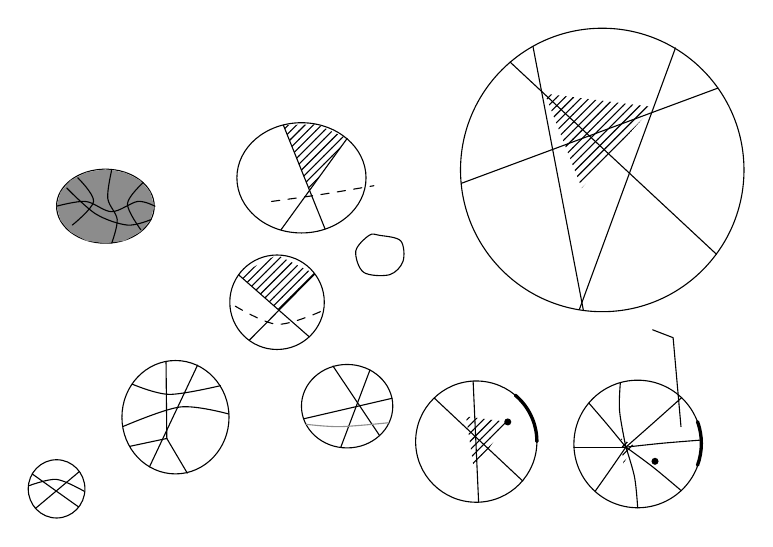
\begin{tikzpicture}[x=1mm,y=1mm,line cap=round,line join=round,font=\scriptsize]
\draw (17.2,-30.3) ellipse[x radius=6.2, y radius=4.7];
\fill[pattern=north east lines,pencil] (23.4,-30.3) -- (22.9,-32.1) -- (21.6,-33.6) -- (19.6,-34.7) -- (17.2,-35) -- (14.8,-34.7) -- (12.8,-33.6) -- (11.5,-32.1) -- (11,-30.3) -- (11.5,-28.5) -- (12.8,-27) -- (14.8,-26) -- (17.2,-25.6) -- (19.6,-26) -- (21.6,-27) -- (22.9,-28.5) -- cycle;
\draw plot[smooth, tension=0.55] coordinates {(11,-30.3) (14.7,-29.7) (18,-31) (21.3,-29.7) (23.5,-30.3)};
\draw plot[smooth, tension=0.55] coordinates {(18,-25.7) (17.5,-29.3) (18.7,-32) (18,-35)};
\draw plot[smooth, tension=0.55] coordinates {(13.7,-26.7) (15.7,-29.7) (13,-32.7)};
\draw plot[smooth, tension=0.55] coordinates {(22,-27.3) (20,-30) (21.7,-33.3)};
\draw plot[smooth, tension=0.55] coordinates {(12.3,-28) (16,-31.3) (20,-32.7) (23,-32)};
\draw (42.1,-26.7) ellipse[x radius=8.2, y radius=7];
\draw (39.8,-20) -- (45.1,-33.2);
\draw (47.9,-21.7) -- (39.5,-33.3);
\fill[pattern=north east lines] (39.8,-20) -- (44,-19.9) -- (47.9,-21.7) -- (43.1,-28.3) -- cycle;
\draw[dashed] plot[smooth, tension=0.55] coordinates {(38.3,-29.7) (44.7,-28.8) (51.3,-27.7)};
\draw plot[smooth cycle, tension=0.55] coordinates {(52,-34) (54.7,-34.7) (55,-37.3) (53.3,-39) (50,-38.7) (49,-36) (50.7,-34)};
\draw (39,-42.5) circle[radius=6];
\draw (34.1,-39) -- (43.1,-46.9);
\draw (43.8,-38.9) -- (35.5,-47.3);
\fill[pattern=north east lines] (34.1,-39) -- (39,-36.5) -- (43.8,-38.9) -- (39.3,-43.5) -- cycle;
\draw[dashed] plot[smooth, tension=0.55] coordinates {(33.7,-43) (39,-45.3) (44.5,-43.7)};
\draw (80.3,-25.7) circle[radius=18];
\draw (68.6,-12) -- (94.8,-36.4);
\draw (71.5,-10) -- (77.9,-43.5);
\draw (89.6,-10.2) -- (77.4,-43.4);
\draw (95,-15.3) -- (62.4,-27.4);
\fill[pattern=north east lines] (73,-16) -- (86.7,-17.7) -- (77.7,-28) -- cycle;
\draw (86.7,-46) -- (89.3,-47) -- (90.3,-58.3);
\draw (11,-66.2) ellipse[x radius=3.6, y radius=3.7];
\draw (7.9,-64.3) -- (13.8,-68.5);
\draw (13.9,-64) -- (8.3,-68.7);
\draw plot[smooth, tension=0.55] coordinates {(7.5,-65.8) (11,-65) (14.5,-66.5)};
\draw (26.1,-57.1) ellipse[x radius=6.8, y radius=7.2];
\draw (24.9,-50) -- (25,-59.8);
\draw (25,-59.8) -- (27.6,-64.2);
\draw (25,-59.8) -- (20.3,-60.8);
\draw (28.9,-50.5) -- (22.8,-63.4);
\draw plot[smooth, tension=0.55] coordinates {(20.6,-52.9) (25.3,-54.2) (31.8,-53.1)};
\draw plot[smooth, tension=0.55] coordinates {(19.4,-58.3) (26.7,-55.8) (32.9,-56.7)};
\draw (47.9,-55.7) ellipse[x radius=5.8, y radius=5.3];
\draw (46.1,-50.6) -- (52,-59.4);
\draw (50.8,-51.1) -- (47.1,-60.9);
\draw plot[smooth, tension=0.55] coordinates {(42.4,-57.3) (48,-56) (53.6,-54.7)};
\draw[pencil] plot[smooth, tension=0.55] coordinates {(42.7,-58) (47,-58.3) (53.2,-57.8)};
\draw (64.3,-60.2) circle[radius=7.7];
\draw (63.9,-52.5) -- (64.6,-67.9);
\draw (59,-54.7) -- (70.2,-65.2);
\fill[pattern=north east lines] (63,-57) -- (68.3,-57.7) -- (64,-63.7) -- cycle;
\node[pt] at (68.3,-57.7) {};
\draw[very thick] (72,-60.2) arc[start angle=0, end angle=50, x radius=7.7, y radius=7.7];
\draw (84.8,-60.5) circle[radius=8.1];
\draw plot[smooth, tension=0.55] coordinates {(83.3,-60.9) (82.5,-56.3) (82.6,-52.7)};
\draw plot[smooth, tension=0.55] coordinates {(83.3,-60.9) (81,-58.1) (78.6,-55.3)};
\draw plot[smooth, tension=0.55] coordinates {(83.3,-60.9) (80,-60.9) (76.7,-60.9)};
\draw plot[smooth, tension=0.55] coordinates {(83.3,-60.9) (81.3,-63.8) (79.4,-66.5)};
\draw plot[smooth, tension=0.55] coordinates {(83.3,-60.9) (84.4,-64.7) (84.8,-68.6)};
\draw plot[smooth, tension=0.55] coordinates {(83.3,-60.9) (86.7,-63.4) (90.3,-66.4)};
\draw plot[smooth, tension=0.55] coordinates {(83.3,-60.9) (88,-60.4) (92.9,-60)};
\draw plot[smooth, tension=0.55] coordinates {(83.3,-60.9) (86.7,-57.9) (90.4,-54.6)};
\fill[pattern=north east lines] (82.7,-59.8) -- (84.3,-60.7) -- (83,-63) -- cycle;
\node[pt] at (87,-62.7) {};
\draw[very thick] (92.4,-63.2) arc[start angle=-20, end angle=20, x radius=8.1, y radius=8.1];
\end{tikzpicture}
\end{document}
